\scanpage{90}
\figure{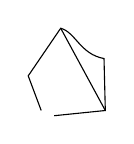
\begin{tikzpicture}[scale=.55]
\draw (0,0)--(-.3,.8)--(.45,1.9) .. controls (.8,1.8) and (.9,1.3) .. (1.45,1.2)--(1.48,0)--(.3,-.12); \draw (.45,1.9)--(1.48,0);
\end{tikzpicture}}
\figure{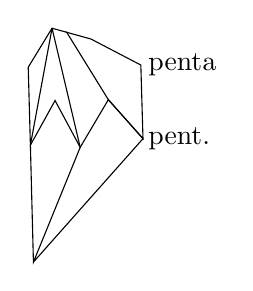
\begin{tikzpicture}[scale=.55]
\draw (0,1.8)--(.55,2.7)--(1.45,2.45)--(2.6,1.85)--(2.65,.15)--(1.85,1.05)--(1.2,-.05)--(.62,1.03)--(.05,0)--(0,1.8);
\draw (.55,2.7)--(.05,0) (.55,2.7)--(1.2,-.05) (.88,2.62)--(1.85,1.05)--(2.65,.15); \draw (.05,0)--(.12,-2.7)--(1.2,-.05) (.12,-2.7)--(2.65,.15);
\node[right] at (2.55,1.85){$\mathrm{penta}$}; \node[right] at (2.55,.15){$\mathrm{pent.}$};
\end{tikzpicture}}
\diagram{\resizebox{\linewidth}{!}{\begin{tikzcd}[ampersand replacement=\&,row sep=1em,column sep=0.65em]

\arrow[from=arc,to=ar,"3"]
\arrow[from=ar,to=seg,"3"]
\arrow[from=arc,to=s,bend left=12]
\arrow[from=dod,to=s,bend right]
\arrow[from=pt,to=s]
\arrow[from=arr,to=db,"2"]
\arrow[from=pt,to=arr]
\arrow[from=car,to=s]
\arrow[from=bp,to=s]
\arrow[from=bp,to=db]
\arrow[from=arr,to=bp]
\arrow[from=cs,to=ca,"2"]
\arrow[from=hs,to=ca,"2"]
\arrow[from=ca,to=car,"2"]
\arrow[from=cs,to=hs,dashed]
\arrow[from=hs,to=car,"\mathrm{car}"]
\arrow[from=hd,to=car,"2"]
\arrow[from=hs,to=htt]
\arrow[from=hdst,to=htt,"2"]
\arrow[from=he,to=cs,"2"]
\arrow[from=he,to=hs,"2"]
\arrow[from=he,to=hdst,"3"]
\arrow[from=he,to=hep]
\arrow[from=he,to=hx,"2"]
\arrow[from=hdst,to=hor,"2"]
\arrow[from=hep,to=hor]
\arrow[from=hs,to=hd,"2"]
\arrow[from=hep,to=hd]
\arrow[from=hor,to=Hsx,"2"]
\arrow[from=hd,to=Hsx,"3"]
\arrow[from=htt,to=Hsx,"2"]
\arrow[from=Hsx,to=s]
\arrow[from=Hsx,to=Hid,"\substack{2\\\mathrm{opp}}"]
\arrow[from=Hid,to=bp]
\arrow[from=Hid,to=H,"3"]
\arrow[from=Hp,to=Hid,"2"]
\arrow[from=HsX,to=Hid,"2"]
\arrow[from=Hsx,to=Htr,"{3\quad u}"]
\arrow[from=He,to=Hsx,"2"]
\arrow[from=hd,to=tri]
\arrow[from=hx,to=hd,"2"]
\arrow[from=hx,to=He,"3"]
\arrow[from=hdst,to=He,"2"]
\arrow[from=tri,to=Htr,"3"]
\arrow[from=Htr,to=H,"\substack{2\\\mathrm{opp}}"]
\arrow[from=HsX,to=H,"2"]
\arrow[from=Hf,to=H,"2"]
\arrow[from=He,to=Htr]
\arrow[from=He,to=HsX,"{2\quad 2}"]
\arrow[from=Hp,to=Ho,"3"]
\arrow[from=HsX,to=Ho,dash]
\arrow[from=Htt,to=Htr,"2"]
\arrow[from=Htt,to=Ho,"2"]
\arrow[from=He,to=Htt,"3"]
\arrow[from=Htt,to=Hf,"2"]
\arrow[from=HsX,to=Hf]
\arrow[from=H,to=TH,"3", "{\deleted{\unsure{\mathrm{triHex}}}\ \deleted{\unsure{(\simeq\mathrm{tripav})}}}"' near end]
\arrow[from=Htr,to=pav,"2"]
\arrow[from=pav,to=TH,"3"]
\arrow[from=bt,to=HsX,dash]
\arrow[from=bt,to=Hid,bend left=9]
 \&  \&  \&  \&  \& |[alias=ca]| \mathrm{Car}_{d*}\simeq\mathrm{pav}+\mathrm{or} \&  \&  \\
 \&  \& |[alias=dod]| \mathrm{dodécép}\simeq\mathrm{pentép}\simeq\mathrm{carrép} \& |[alias=ar]| \substack{\mathrm{Ar}\\{}\simeq\unsure{\mathrm{segpté}|\mathrm{trig\,pt}}} \& |[alias=arc]| \substack{\mathrm{Arc}\\{}\simeq\unsure{\mathrm{segép}|\mathrm{trig\,ép}}} \&  \&  \&  \\
 \&  \&  \& |[alias=seg]| \unsure{\mathrm{seg}}\deleted{\unsure{p}} \&  \&  \&  \&  \\
 \& |[alias=pt]| \mathrm{pent.} \& |[alias=s]| S \&  \&  \& |[alias=car]| \mathrm{car} \&  \& |[alias=cs]| \mathrm{car}_{s*} \\
|[alias=arr]| \unsure{\mathrm{arête}} \&  \&  \& |[alias=htt]| \substack{\mathrm{hex}_{tt*}\\(\simeq\mathrm{pav}+\mathrm{or}\\{}+\mathrm{tria})} \&  \&  \& |[alias=hs]| \substack{\mathrm{hex}_{s*}\simeq\mathrm{car}_{\unsure{t'|r}}\\(\simeq\mathrm{pav}+\mathrm{tria}+\mathrm{or})} \&  \\
|[alias=db]| \substack{\unsure{\mathrm{db\;point}|\mathrm b}\simeq\mathrm{doublet}\\\deleted{\unsure{\mathrm{ob\;arête}}}} \&  \&  \&  \& |[alias=hdst]| \substack{\mathrm{hex}_{\unsure{d*|\Omega*}}\;\deleted{\unsure{b}}\\\unsure{\mathfrak S_3|G_3}} \&  \&  \& |[alias=he]| \substack{\mathrm{hexép}\simeq\mathrm{carép}\\(\simeq\mathrm{pavép})\;(\mathrm G_{\mathrm{pav}})\\(\simeq\mathrm{carép})} \\
 \&  \&  \& |[alias=hor]| \substack{\mathrm{hexor}\\\mathfrak S_3} \&  \&  \& |[alias=hep]| \substack{\mathrm{hexép}'\\(\mathfrak S_3)} \&  \\
|[alias=bp]| \unsure{\mathrm{bi\;pct}|\mathrm{bi\,pt}} \& |[alias=Hid]| \substack{\mathrm{Hex}_{id}^{*}\\(\simeq\mathrm{tria})} \&  \& |[alias=Hsx]| \substack{\mathrm{Hex}_s\simeq\mathrm{hex}\\(\simeq\mathrm{tria})} \&  \& |[alias=hd]| \substack{\mathrm{hex}_{d}\quad\mathfrak S_2\\{}\simeq\mathrm{tria\;pct}\\{}\simeq\mathrm{car}_d} \&  \&  \\
 \&  \& |[alias=Hp]| (\mathbb D_3)\,\mathrm{Hexép}' \&  \&  \&  \&  \&  \\
 \& |[alias=H]| \substack{\mathrm{Hex}\\(\simeq\mathrm{pav})} \&  \& |[alias=Htr]| \substack{(\mathbb D_3)\,\mathrm{Hex}_{tr}\\(\simeq\mathrm{tritria})} \&  \& |[alias=tri]| \mathrm{tria} \&  \&  \\
|[alias=bt]| \unsure{\mathrm{b.}} \&  \& |[alias=HsX]| \substack{\mathrm{Hex}_{s*}\\(\simeq\unsure{\mathrm{bapl}|\mathrm{bapt}|\mathrm{ba\,pt}})} \&  \& |[alias=He]| \substack{(\mathbb D_6)\,\mathrm{Hexép}\simeq\mathrm{hex}_{tr}\\(\simeq\mathrm{trép\,tria})\quad\mathfrak S_3} \&  \&  \& |[alias=hx]| \substack{\mathrm{hex}_{s}\simeq\mathrm{car}_{s}\\(\simeq\mathrm{triaép})\quad\mathfrak S_3} \\
 \&  \&  \& |[alias=Ho]| \mathrm{Hexor} \&  \&  \&  \&  \\
 \&  \& |[alias=Hf]| \substack{\mathrm{Hex}_{t*}\\(\simeq\mathrm{triba})} \&  \& |[alias=Htt]| \substack{\mathrm{Hex}_{tt*}\;(\mathbb F_2\times\mathbb F_2)\\(\simeq\mathrm{trortria})} \&  \&  \&  \\
 \& |[alias=TH]| \substack{\mathrm{triHex}\\(\simeq\mathrm{tripav})} \&  \& |[alias=pav]| \mathrm{pav} \&  \&  \&  \& 
\end{tikzcd}}}
% slanted
\margin{\unsure{investiguer|inventorier|invariants} cube et hypercube dans \unsure{domaine|divers domaines|domaines} \deleted{\unsure{questions}} polyèdres et polyt. \unsure{prod.|pro\ldots}}
\[
\left(\mathrm{prismes}\ \left\{\begin{array}{l}
\text{triangulaires}\\\text{pentagonaux}\\\text{hexagonaux}
\end{array}\right.\right.
\]
produit de polygones\ldots
\figure{\begin{tikzpicture}[x=8mm,y=5mm]\draw[->] (4,2.2) to[bend right=25] (0,0);\draw[->] (4.8,1.7) to[bend left=38] (1,-.9);\end{tikzpicture}}

% slanted
\margin{\tikz[baseline=(a.base)]{\node (a){étranges !};\draw (a.center) ellipse (1.1cm and .34cm);}}
\diagram{\begin{tikzcd}[ampersand replacement=\&,row sep=1.0em]
{} \arrow[d] \& {} \arrow[l] \& {}\\
\bullet \& {} \arrow[ul] \& {} \arrow[ul]\\
{} \& \circ \arrow[ul,dashed] \arrow[uu] \arrow[dd] \& {}\\
{} \& {} \& {} \arrow[uu] \arrow[ul,dash] \arrow[dd]\\
{} \& \bullet \arrow[uuul] \& {}\\
{} \& {} \& {} \arrow[ul]
\end{tikzcd}}
\figure{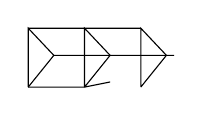
\begin{tikzpicture}[scale=.65]
\foreach \x in {0,1.1,2.2}{\draw (\x,0)--(\x,1.15)--(\x+.5,.62)--(\x,0);}
\draw (0,1.15)--(2.2,1.15) (0,0)--(1.1,0)--(1.6,.1) (.5,.62)--(2.85,.62);
\end{tikzpicture}}
\figure{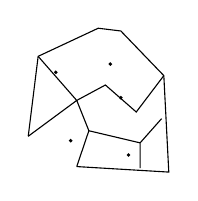
\begin{tikzpicture}[scale=.7]
\draw (0,0)--(.18,1.45)--(1.27,1.96)--(1.68,1.91)--(2.46,1.1)--(2.55,-.65)--(.88,-.55);
\draw (.18,1.45)--(.88,.65)--(1.1,.1)--(.88,-.55) (0,0)--(.88,.65)--(1.4,.93)--(1.96,.44)--(2.46,1.1) (1.1,.1)--(2.03,-.12)--(2.42,.32) (2.03,-.12)--(2.03,-.58);
\foreach \p in {(.5,1.16),(1.49,1.31),(1.68,.7),(.77,-.08),(1.82,-.34)}\fill \p circle(1pt);
\end{tikzpicture}}
% archive sheet number: 89
